\section{Směrování} \label{prijmiEthernetove}
Směrování implementoval kolega, nicméně Cisco se nechová vždy stejně, a tak bylo nutné vyčlenit rozhodování o~příjmu paketů do koncových počítačů a implementovat je každý zvlášť. Nejsložitější bylo zjistit, jak se cisco přesně chová a proč. Všechny vyzkoumané informace byly platné v~období březen - duben 2010. Někdo předělával školní cisca po tom, co jsem prováděl experimenty, takže je možné, že některé věci se mohou chovat jinak (nové verze IOS či jen jiná konfigurace). 

Při různých experimentech jsem zjistil, že když linuxu přijde paket, na který nemá záznam ve směrovací tabulce, tak pošle zpátky patek \verb|Destination Network Unreachable|, zatímco školní cisca posílají \verb|Destination Host Unreachable|.

Při testování standardních případů je vše jasné, ale když jsem zkusil nakonfigurovat síť trochu neobvykle, tak to tak jasné nebylo. Experimenty byly ověřovány pomocí příkazu \verb|ping|, který implementoval kolega\footnote{viz kapitola vymezení spolupráce \ref{vymezeni}}. 

%------------------------------------------------------------------------------

\subsection{Debuging}
Na stránkách firmy Cisco Systems jsem objevil několik návodů týkajících se vypisování zpracování paketů na jednotlivých strojích. Bez těchto návodů lze jen těžko hádat, které pakety se posílají kam. Velmi užitečné jsou příkazy, které poskytují detailní výpis aktuálně zpracovávaných paketů:

\begin{itemize}
 \item \verb|debug ip packet detail| - IP pakety 
 \item \verb|debug ip icmp| - ICMP\footnote{Internet Control Message Protocol je jeden z~nejdůležitějších protokolů ze sady protokolů internetu. Používají ho operační systémy počítačů v~síti pro odesílání chybových zpráv, například pro oznámení, že požadovaná služba není dostupná nebo že potřebný počítač nebo router není dosažitelný. \cite{wiki:icmp}} pakety
 \item \verb|debug arp| - ARP pakety
\end{itemize}

%------------------------------------------------------------------------------

\subsection{Síť č.1}
\subsubsection{Popis problému}
Síť na obrázku \ref{fig:sit_2pc} je složená pouze ze dvou počítačů cisco a linux. Tyto počítače mají nastavené IP adresy z~jiných sítí, linux má nastavený defaultní záznam na rozhraní \verb|eth0| a cisco má samo-nastavující se záznam na síť, která je připojena na rozhraní \verb|F0/0|\footnote{Na obrázcích sítí se vyskytují zkratky F0/0 a F0/1, které značí FastEhernet0/0 resp. FastEhernet0/1}. Samo-nastavující znamená, že cisco přidává záznamy do routovací tabulky podle IP adresy z~jeho rozhraní. Tuto funkcionalitu lze vypnout, na školních ciscách je ale defaultně zapnutá. Cisco nepřidává tento záznam v~případě, že na druhém konci kabelu buď nikdo není nebo je rozhraní shozené (vypnuté).

\begin{figure}[h]
\begin{center}
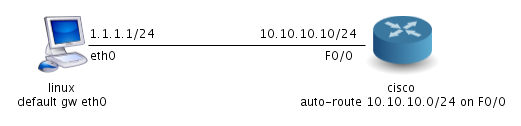
\includegraphics[width=13cm]{figures/sit_2pc.png}
\caption{Síť linux - cisco}
\label{fig:sit_2pc}
\end{center}
\end{figure}

Při připojení na linux a spuštění příkazu \verb|ping 10.10.10.10| se stane, že u~prvních pár paketů (při mém testování to bylo 9) vyprší timeout a pak už linux sám sobě vypisuje \verb|Destination Host Unreachable|. Dlouho jsem se snažil přijít na to, proč to tak je. Těžko jsem zjišťoval, co se děje, protože jsem neměl žádné zkušenosti se sledováním paketů přes cisco směrovače. 

\subsubsection{Řešení} 
Nejdříve vysvětlím proč prvních několik paketů prošlo až na cisco a na další \verb|icmp_req| odpověděl linux sám sobě. Je to způsobeno tím, že při prvních paketech ještě cisco nevědělo co s~těmi pakety bude, a tak je přijalo, aby mohlo vyhodnotit co dál. Cisco ale hned přišlo na to, že nemá žádný záznam na \verb|1.1.1.1|, takže neví, co s~takovými pakety dělat, tak se radši rozhodlo, že je ani nepřijme. Obvykle cisco nepřijímá pakety hned od začátku, když nemá záznam pro takový paket, ale školní cisca mají starší verzi software a celkově reagují trochu pomaleji, než je zvykem, takže to moho být způsobeno tím.

\paragraph{Průchod ARP žádostí}
Linux nejprve pošle ARP request, aby zjistil MAC adresu cisca. Cisco přijme ARP request a snaží se odpovědět (poslat ARP reply). Problém je, že nemá záznam v~routovací tabulce na adresu \verb|1.1.1.1|, takže ani neodpoví na ARP request, tak \uv{hezky} je nastavené cisco.

Po přidání záznamu \verb|ip route 1.1.1.0 255.255.255.0 F0/0| do routovací tabulky na směrovači \verb|cisco| síť funguje bez jakýchkoliv problémů. Do této chvíle jsem netušil, že je něco takového možné. A~ono stačí správně nastavit směrovací záznamy na obou počítačích.

%------------------------------------------------------------------------------

\subsection{Síť č.2}
\subsubsection{Popis sítě}
Na další síti \ref{fig:sit_3pc} jsou počítače linux1, cisco1 a cisco2 zapojené v~jednom řetězu. Konfigurace rozhraní a směrovacích tabulek je vepsána v~obrázku. Linux1 má teoreticky v~dosahu (přes defaultní záznam) cisco2, to mu ale nemůže odpovědět, protože pro linux1 nemá záznam. Cisco1 přeposílá pakety z~cílovou adresu \verb|8.8.8.0/24| na bránu - cisco2.

\begin{figure}[h]
\begin{center}
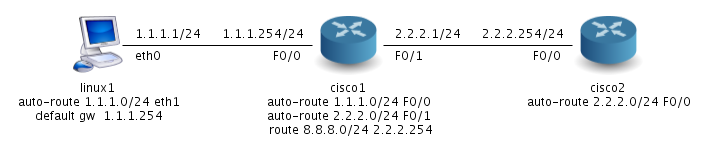
\includegraphics[width=15cm]{figures/sit_3pc.png}
\caption{Síť linux1 - cisco1 - cisco2}
\label{fig:sit_3pc}
\end{center}
\end{figure}

%------------------------------------------------------------------------------

\newpage

\subsubsection{Experimenty} 

\paragraph{I. experiment}
První experiment je \verb|ping| z~linux1 směrem na cisco2:
\begin{verbatim}
linux1:/home/dsn# ping -c2 8.8.8.8
PING 8.8.8.8 (8.8.8.8) 56(84) bytes of data.

--- 8.8.8.8 ping statistics ---
2 packets transmitted, 0 received, 100% packet loss, time 1006ms
\end{verbatim}

Vše dopadlo dle očekávání tedy paket proplul až na vzdálené cisco2, které nemělo pravidlo pro manipulaci paketů s~cílem \verb|8.8.8.8|, a tak chtělo poslat zpátky odesílateli \\\verb|Destination Host Unreachable|. Problém je, že cisco2 nemá záznam ve směrovací tabulce pro zdrojovou adresu \verb|1.1.1.1| (linux1), takže vyprší timeout, protože nelze doručit odpovědět o~nedoručení.

Po přidání záznamu pro obsluhu sítě \verb|1.1.1.0/24| na bránu \verb|2.2.2.1| na směrovači cisco2, tak vše už funguje dle očekávání:
\begin{verbatim}
linux1:/home/dsn# ping -c2 8.8.8.8
PING 8.8.8.8 (8.8.8.8) 56(84) bytes of data.
From 2.2.2.254 icmp_seq=1 Destination Host Unreachable
From 2.2.2.254 icmp_seq=2 Destination Host Unreachable
\end{verbatim} 


\paragraph{II. experiment}
Pokud zkusíme odeslat \verb|ping| na \verb|1.1.1.2|, což je adresa v~síti mezi linux1 a cisco1, ale není to adresa ani jednoho z~nás, tak dopadne takto:
\begin{verbatim}
linux1:/home/dsn# ping -c2 1.1.1.2
PING 1.1.1.2 (1.1.1.2) 56(84) bytes of data.
From 1.1.1.1 icmp_seq=1 Destination Host Unreachable
From 1.1.1.1 icmp_seq=2 Destination Host Unreachable
\end{verbatim} 
Linux ví (díky ARP protokolu), že vedle něj není počítač s~IP adresou \verb|1.1.1.2|, a tak se to ani nesnaží odeslat a odpovídá sám sobě, že je host nedostupný. 


\paragraph{III. experiment}
Cisco má trochu odlišné chování:
\begin{verbatim}
cisco1#ping 1.1.1.2

Type escape sequence to abort.
Sending 5, 100-byte ICMP Echos to 1.1.1.2, timeout is 2 seconds:
.....
Success rate is 0 percent (0/5)
\end{verbatim}
Cisco se zeptalo ethernetově (přes ARP) linuxu, ten odpověděl, že takovou adresu nemá a cisco vypsalo '.', což znamená, že vypršel timeout (dle \cite{cisco:icmp_codes}). Zatímco linux poslal \verb|DHU|\footnote{Destination Host Unreachable}.

%------------------------------------------------------------------------------

% \newpage

\subsection{ARP protokol} \label{arp}
\textit{\uv{Address Resolution Protocol (ARP) se v~počítačových sítích s~IP protokolem používá k~získání ethernetové MAC adresy sousedního stroje z~jeho IP adresy. Používá se v~situaci, kdy je třeba odeslat IP datagram na adresu ležící ve stejné podsíti jako odesílatel. Data se tedy mají poslat přímo adresátovi, u~něhož však odesilatel zná pouze IP adresu. Pro odeslání prostřednictvím např. Ethernetu ale potřebuje znát cílovou ethernetovou adresu.}} \cite{wiki:arp}

Z~různých experimentů jsem sestavil tato ARP pravidla, podle kterých cisco vyhodnocuje ARP requesty:
\begin{enumerate}
 \item zdrojová IP adresa není ve stejné síti viz obrázek \ref{fig:sit_2pc}, tak se diskartuje ARP request - lze obejít v~konfiguraci (jako např. na školních směrovačích)
 \item cílová IP adresa nesedí s~žádnou s~žádnou mojí IP adresou, tak se diskartuje ARP reply
 \item IP zdroje (tazatele) je dostupná přes pravidla v~routovací tabulce, tak se vygeneruje ARP reply a pošle se tazateli
\end{enumerate}

%------------------------------------------------------------------------------

\subsection{Pravidla o~příjmu paketů} 
Z~předchozí sekce \ref{arp} jsem odvodil několik pravidel pro příjem paketů u~cisco směrovače. Tato pravidla tvoří de facto tělo metody \verb|prijmiEthernetove| u~\verb|CiscoPocitac|.

\begin{itemize}
 \item když mohu odpovědět na ARP request a zároveň je paket pro mě nebo vím kam ho poslat dál, tak se paket přijme
 \item když nelze odpovědět na ARP request = nemám na něj záznam ve směrovací tabulce, tak se paket nepřijme
 \item ve všech ostatních případech se paket nepřijme
\end{itemize}



